% -*- coding: utf-8 -*-
% !TEX program = xelatex

%\documentclass[11pt,a4paper]{article}
\documentclass[12pt,final]{article}

\usepackage[UTF8]{ctex}
\usepackage{amsmath,amsthm,amssymb}
\usepackage{mathrsfs}
\usepackage{graphicx}
\usepackage{subfig}
%\usepackage[english]{babel}
\usepackage{color,xcolor}
\usepackage{enumitem}
\usepackage{lipsum} % 用于生成示例文本
\usepackage{float}
\usepackage{pifont}
\usepackage{tabularx}
\usepackage{booktabs}
\usepackage{array}
\usepackage{multirow,multicol}
\usepackage{longtable}
\usepackage{makecell}
\usepackage{anyfontsize}
%\usepackage{microtype}
\usepackage{geometry}
\usepackage{relsize} % For smaller command
%\geometry{left=1.25in,right=1.25in,top=1in,bottom=1in}
\geometry{left=3cm,right=3cm,top=3cm,bottom=3cm}
\setlength{\headheight}{18pt}
\setlength{\headsep}{18pt}
\setlength{\footskip}{25pt}

%----- 设置超链接 -----
\usepackage{hyperref}
\usepackage{cleveref}
\hypersetup{
	colorlinks=true,
	linkcolor=black,
	citecolor=blue,
	filecolor=blue,
	urlcolor=blue
}

% 允许多行公式跨页显示
\allowdisplaybreaks

%----- 定义页眉-----
\makeatletter
\newcommand\@header{}
\newcommand\header[1]{\def\@header{#1}}
\makeatother

%----- 页眉页脚 -----
\usepackage{fancyhdr}
\makeatletter
\pagestyle{fancy}
\fancyhf{}
\fancyhead[C]{\small\kaishu\@header}
\fancyfoot[C]{\small\thepage}
\renewcommand{\headrulewidth}{0.5pt}
\makeatother

%----- 设置英文字体 -----
%\usepackage[no-math]{fontspec}
%\usepackage{newtxtext}  % New TX font for text
%\setmainfont{TeX Gyre Termes}  % Times New Roman 的开源复刻版本
%\setsansfont{TeX Gyre Heros}   % Helvetica 的开源复刻版本
%\setmonofont{TeX Gyre Cursor}  % Courier New 的开源复刻版本
%\setmainfont{Times New Roman}
%\setsansfont{Arial}
%\setmonofont{Courier New}

%----- 设置数学字体 -----
%\usepackage{newtxmath}
%\usepackage{mathptmx}

%----- 设置编号格式 -----
\numberwithin{equation}{section}
\numberwithin{figure}{section}
\numberwithin{table}{section}

%----- 重新设置图表公式 autoref -------
\renewcommand{\figureautorefname}{图}
\renewcommand{\tableautorefname}{表}
\renewcommand{\equationautorefname}{公式}

%----- 设置各种间距 -----
%\renewcommand{\baselinestretch}{1.35}
%\setlength{\parindent}{2em}
%\ziju{0.1}  % 控制中文字间距
%\setlength{\parskip}{3pt plus1pt minus1pt}

%----- 算法环境 -----
\usepackage{algorithm}
\usepackage{algpseudocode}
\floatname{algorithm}{算法}
\algrenewcommand\algorithmicrequire{\textbf{输入:}}
\algrenewcommand\algorithmicensure{\textbf{输出:}}

%----定义列表项的样式 -----
\usepackage{enumitem}
\setlist{nolistsep}

%-----设置图片的路径 -----
\graphicspath{{./figure/}{./figures/}}

%----- 使用 tabularx库并定义新的左右中格式 -----
\newcolumntype{L}{X}
\newcolumntype{C}{>{\centering \arraybackslash}X}
\newcolumntype{R}{>{\raggedleft \arraybackslash}X}
\newcolumntype{P}[1]{>{\centering \arraybackslash}p{#1}}

%----- 数学定理设置 -----
\theoremstyle{plain}
\renewcommand{\proofname}{证明}
\newtheorem{Theorem}{定理}[section]   % [section] 表示按章节编号
\newtheorem{Lemma}[Theorem]{引理}      % [Theorem] 表示与定理共享编号
\newtheorem{Corollary}[Theorem]{推论}  % [Theorem] 表示与定理共享编号
\newtheorem{Proposition}[Theorem]{性质} % [Theorem] 表示与定理共享编号
\newtheorem{Assumption}[Theorem]{假设} % [Theorem] 表示与定理共享编号
\theoremstyle{Definition}
\newtheorem{Definition}[Theorem]{定义}  % [Theorem] 表示与定理共享编号
\newtheorem{Example}[Theorem]{例}       % [Theorem] 表示与定理共享编号
\theoremstyle{Remark}
\newtheorem{Remark}[Theorem]{备注}      % [Theorem] 表示与定理共享编号

% 自定义标签名称
\crefname{Theorem}{定理}{定理}
\Crefname{Theorem}{定理}{定理}
\crefname{Lemma}{引理}{引理}
\Crefname{Lemma}{引理}{引理}
\crefname{Corollary}{推论}{推论}
\Crefname{Corollary}{推论}{推论}
\crefname{Proposition}{命题}{命题}
\Crefname{Proposition}{命题}{命题}
\crefname{Assumption}{假设}{假设}
\Crefname{Assumption}{假设}{假设}
\crefname{Definition}{定义}{定义}
\Crefname{Definition}{定义}{定义}
\crefname{Example}{示例}{例}
\Crefname{Example}{示例}{例}
\crefname{Remark}{备注}{备注}
\Crefname{Remark}{备注}{备注}
\crefname{figure}{图}{图}
\Crefname{figure}{图}{图}
% 自定义 cref 对 equation 环境的标签格式,仅显示编号
\crefformat{equation}{(#2#1#3)}
\crefrangeformat{equation}{(#3#1#4)--(#5#2#6)}


\makeatletter
\renewenvironment{proof}[1][\proofname]{\par
	\pushQED{\qed}%
	\normalfont \topsep6\p@\@plus6\p@\relax
	\trivlist\item[\hskip\labelsep
	\bfseries #1\@addpunct{\,:\,}]\ignorespaces
}{%
	\popQED\endtrivlist\@endpefalse
}
\makeatother

%----- 参考文献格式 -----
%\bibliographystyle{plain} % abbrv,unsrt,siam
\bibliographystyle{thuthesis-numeric}
%\bibliographystyle{thuthesis-author-year}

%----- 参考文献引用格式 -----
\usepackage[numbers,sort&compress]{natbib}
%\usepackage[numbers,super,square,sort&compress]{natbib}
\def\bibfont{\small}  % 修改参考文献字体
\setlength{\bibsep}{7pt plus 3pt minus 3pt}  % 调整参考文献间距

%----- 微分符号 -----
\newcommand{\dif}{\mathop{}\!\mathrm{d}}

%----- 定义新命令 -----
\newcommand{\CC}{\ensuremath{\mathbb{C}}}
\newcommand{\RR}{\ensuremath{\mathbb{R}}}
\newcommand{\abs}[1]{\lvert#1\rvert}
\newcommand{\norm}[1]{\lVert#1\rVert}
\newcommand{\dx}[1][x]{\mathop{}\!\mathrm{d}#1}
\newcommand{\ii}{\mathrm{i}\mkern1mu} % imaginary
\newcommand{\refe}[2]{(\ref{#1})--(\ref{#2})}
\newcommand{\A}{\mathcal{A}}
\newcommand{\bA}{\boldsymbol{A}}
\newcommand{\red}[1]{\textcolor{red}{#1}}

%----- 论文信息 -----
\header{时间变换随机微分方程的$\alpha$阶逼近}

\title{时间变换随机微分方程的$\alpha$阶逼近}
\author{左如春}
\date{\today}


\begin{document}
	
	\maketitle
	
	\begin{abstract}
		研究Euler-Maruyama (EM)数值逼近一类经过Lamperti变换后,漂移系数线性增长、扩散系数是常数的时变随机微分方程. 证明了EM的强收敛性与逆从属的稳定指数之间的关系,并讨论收敛速度. 并通过数值模拟验证了理论结果. 
		
		\medskip
		\noindent\textbf{关键词:} 时间变换;等距离散;收敛阶;逆从属. 
	\end{abstract}
	
	\section{引言}
	
	受到\cite{Alfonsi2013602}的启发,本文的目的是推导出一个有效的数值逼近具有全局Lipschitz的漂移系数和扩散项系数的一维随机微分方程. 主要思想是使用Lamperti变换将原始的时变SDE转化成带有加性噪声的时变SDE,见\cite{iacus2008simulation},通过EM对变换后的时变SDE进行逼近,再将其变换成原始时变SDE的逼近格式. 
	
	对于时间变换的随机微分方程,现在已经有了很多的数值逼近格式. 在\cite{jum2014strong}中证明了对于漂移项和扩散项都满足全局Lipschitz时,可以采用对偶原则,将时间变换随机微分方程转换成一般随机微分方程,通过对一般随机微分方程使用EM数值格式进行逼近,进而得到时间变换随机微分方程的强收敛阶. 在\cite{deng2020semi}中将这一思想运用在漂移项满足非全局Lipschitz条件时,使用半隐式EM得到强收敛阶,并研究了其稳定性. 这解决了一大类可以对偶化的时间变换微分方程的数值格式收敛性问题. 在\cite{jin2019strong},对于不能使用对偶原则的时间变换随机微分方程,采用一种非等距的离散格式,并得到强收敛阶. 纵观以往的时间变换的随机微分方程的数值格式,大多采用的是非等距离散. 而在这篇文章中,我们将使用等距离散来研究具有全局Lipschitz系数的漂移项系数和常数项扩散项系数的随机微分方程:
	\begin{equation}\label{basic SDE}
		dX(s)=f(X(s))dE(s)+\sigma dB(E(s)). 
	\end{equation}
	
	\section{准备工作}
	
	在这篇文章中, ($\Omega,\mathcal{F},\mathbb{P}$) 表示完备概率空间 , $D=(D(t))_{t\geq0}$ 表示具有Laplace指数$\psi$, 从0开始的从属,其中$\psi$的被杀率是0且具有Lévy测度$\nu;$ 即$D$是具有开始于0的càdlàg路径的一维非减Lévy过程,其Laplace变换是:
	$$\mathbb{E}[e^{-sD(t)}]=e^{-t\psi(s)},\quad\text{其中}\quad\psi(s)=\int\limits_0^\infty(1-e^{-sy})\:\nu(\text{d}y),\quad s>0.$$
	并且 $\int_0^\infty(y\wedge1)\nu(dy) < \infty$,
	我们考虑Lévy测度$\nu$是无穷的情况,即$\nu ( 0,\infty ) = \infty$.这意味着复合泊松从属不在我们的考虑范围中. 令 $E=(E(t))_{t\geq0}$是$D$的逆,即:
	$$E(t):=\inf\{s>0;D(s)>t\},\:t\geq0. $$
	我们称$E$是逆从属过程,注意$E$是连续且非递减的. 如果从属 $D$ 是Laplace指数为$\psi(s) = s^{\beta}$, $\beta \in (0,1)$的稳定过程,那么对应的 $E$ 称为逆 $\beta$-稳定从属过程. 一般我们假设$B(t)$ 和 $D(t)$ 是相互独立的. 随机过程$B(E(t))$被称作时间变换的布朗运动. 我们注意到$D(t)$的跳跃部分和$E(t)$的平坦部分相互对应的. 又由于$E(t)$的平坦部分,导致$B(E(t))$在这一部分也是平坦的,因此$B(E(t))$可以被理解成是一种次扩散. 
	
%	令 $S=(l,r)$,其中 $-\infty\leq l<r\leq\infty$,函数 $a,b$是$S\to S$ 的连续可微函数. 考虑下面的SDE:
%	$$dy(t)=a(y(t))dE(t)+b(y(t))dB(E(t)),\quad t\geq0,\quad y(0)\in S$$
%	并且假设它在S中有唯一强解,即
%	$$\mathbb{P}(y(t)\in S,\:t\geq0)=1. $$
%	如果 $b(x)>0$ 对所有的 $x\in S$都成立,那么我们可以使用Lamperti变换
%	$$F(x)=\lambda\int^x\frac1{b(y)}dy$$
%	对于某些$\lambda>0. $并且$F^{-1}:F(S)\to S$ 是被良好定义的,令$x(t)=F(y(t))$利用\cite{umarov2018beyond}中的时间变换It\^{o}公式可以得到:
%	$$dx(t)=f(x(t))dE(t) + \lambda dB(E(t)) \quad t\geq0,\quad x(0)\in F(S)$$
%	其中
%	$$f(x)=\lambda\left(\frac{a(F^{-1}(x))}{b(F^{-1}(x))}-\frac12b^{\prime}(F^{-1}(x))\right),\quad x\in F(S),$$
%	$F(D)=(F(l),F(r)). $ 这种变换可以将扩散项的非线性项转换到漂移项中. 
	令 $S=(l,r)$,其中 $-\infty\leq l<r\leq\infty$,函数 $f$是$S\to S$ 的连续可微函数. 考虑SDE\cref{basic SDE}
	并且假设它在S中有唯一强解,即
	$$\mathbb{P}(X(t)\in S,\:t\geq0)=1. $$
	
	设定等距步长 $\delta \in (0,1)$ 及时间区间 $T > 0$. 为了在区间 $[0,T]$ 上逼近逆从属过程 $E$,我们遵循 \cite{magdziarz2009stochastic} 中提出的方法. 具体来说,首先通过模拟具有独立且平稳增量的从属过程 $D$ 的样本路径来进行逼近. 设定 $D_0 = 0$,然后遵循规则 $D_{i\delta} := D_{(i-1)\delta} + Z_i,i=1,2,3,\ldots$,其中 $\{Z_i\}_{i \in \mathbb{N}}$ 为独立同分布的序列,且 $Z_i \stackrel{d}{=} D_{\delta}$. 我们在找到整数 $N$ 使得 $T \in [D_N\delta,D_{(N+1)\delta})$ 时停止该过程. 请注意,$\mathbb{N}\cup\{0\}$ 值的随机变量 $N$ 确实存在,因为 $D_t \to \infty$ 随着 $t \to \infty$ 几乎必然成立. 可以通过下面的算法生成随机变量 $\{Z_i\}$,
	\begin{align*}
		Z(i)=\delta^{1/\alpha}\xi_{i},
	\end{align*}
	其中$\xi_i$是独立同分布的完全偏斜的$\alpha$稳定随机变量, $\xi_i$的实现过程如下:
	\begin{align*}
		\xi_i=\frac{\sin(\alpha(V+c_1))}{\left(\cos(V)\right)^{1/\alpha}}\Big(\frac{\cos(V-\alpha(V+c_1))}{W}\Big)^{(1-\alpha)/\alpha},
	\end{align*}
	其中$c_1 = \frac{\pi}{2}$,随机变量$V$是$(-\frac{\pi}{2},\frac{\pi}{2})$上的均匀分布, $W$是均值为$1$的指数分布. 
	然后,令
	$$
	E_t^\delta := \left(\min\{n \in \mathbb{N}; D_{n\delta} > t\} - 1\right)\delta,\quad t \in [0,T]. 
	$$
	过程 $E^\delta = (E_t^\delta)_{t \geq 0}$ 的样本路径是具有恒定跳跃大小 $\delta$ 的单调递增阶梯函数,第 $i$ 个等待时间为 $Z_i = D_{i\delta} - D_{(i-1)\delta}$. 过程 $E^\delta$ 有效地逼近 $E$;实际上,几乎必然地有
	$$
	E_t - \delta \leq E_t^\delta \leq E_t ,~~\text{对于所有} 的 t \in [0,T]. 
	$$
	
	\cref{fig1}中提供在这种离散方式下的$E(t)$和$X(t)$. 在\cite{jin2019strong}中对$\Delta E$的处理时, t每次跳$D_{n\delta} - D_{(n-1)\delta}$, 于是$E(t)$每次对应改变$\delta$. 然而,在我们的离散格式中,选择对t做等距离散,让t每次跳跃的长度是固定的长度h,于是$E$在第i次跳跃对应的变化就是$E_{ih} - E_{(i-1)h}$,这样的离散会导致出现$\Delta E=0$,这是得到收敛阶是$\alpha$的关键. 
	\begin{figure}[htp!]
		\centering
		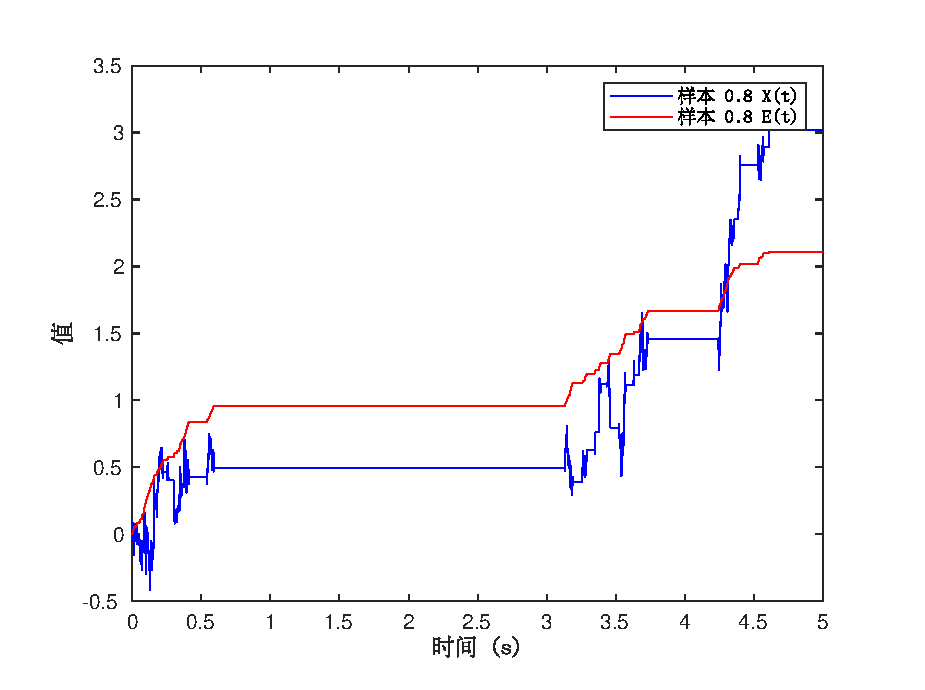
\includegraphics[width=0.6\linewidth]{EandX.eps}
		\caption{$E(t)$和$X(t)$的样本路径.}
		\label{fig1}
		\vspace{-2ex}
		{}
	\end{figure}
	
	
	\section{假设和引理}
	\begin{Assumption}\label{assum1}
		假设函数$f$满足全局\textnormal{Lipschitz}条件的,即存在一个常数$K>0$, 使得:
		\begin{equation}
			|f(x)-f(y)| \le K|x-y|.
		\end{equation}
	\end{Assumption}
	
	\begin{Assumption}\label{assum2}
		令T>0,假设函数$f$是二阶连续可微的并且满足:
		\begin{equation}
			\sup\limits_{t\in[0,T]}\mathbb{E}\left|f'(x(t))\right|^2+
			\sup\limits_{t\in[0,T]}\mathbb{E}\left|f'(x(t))f(x(t))+
			\frac{\sigma^2}2f''(x(t))\right|<\infty. 
		\end{equation}
	\end{Assumption}
	
	\begin{Lemma}\label{Lemma:1}
		令$\Delta t > 0,~g_n,~\lambda _n \in \mathbb{R},~\eta > 0$,~$a_0=0$,~再假设$1-\eta \Delta t > 0$,~$1 + \lambda _n > 0,~n \in \mathbb{N}$,~那么如果
		\begin{equation*}
			a_{n+1} \leq a_n(1+\lambda _n)+\eta a_{n+1}\Delta t +g_{n+1},
		\end{equation*}
		则下面的不等式成立:
		\begin{equation}
			a_n \leq \frac{1}{(1-\eta\Delta t)^n}\sum\limits_{j=0}^{n-1}(1-\eta\Delta t)^jg_{j+1}\prod\limits_{l=j+1}^{n-1}(1+\lambda _l).
		\end{equation}
	\end{Lemma}
	
	
	可以在\cite{umarov2018beyond}中得到下面的时间变换的It\^{o}公式. 
	\begin{Lemma}\label{ito}
		令 B 是一维标准的布朗运动. 令 $D$ 和 $E$满足 $[ D\longrightarrow E]$ 或者 $[ U\longleftarrow E]. $ X是由下述\textnormal{SDE}定义的随机过程
		$$X{(t)}:=\int_0^tA{(s)}ds+\int_0^tF{(s)}dE{(s)}+\int_0^tG{(s)}dB_{E{(s)}},$$
		其中 $A\in$ $L( t,\mathcal{F} _{E{(t)}})$,$F\in$ $L( E{(t)},\mathcal{F} _{E{(t)}})$,以及 $G\in$ $L( B_{E{(t)}},~\mathcal{F} _{E{(t)}}) . ~$ 如果 $f\in$ $C^2( \mathbb{R} )$,~那么
		$f(X(t))$ 是$\mathcal{F}_{E{(t)}}-$半鞅, 对于所有的t $\ge$ 0, 都有
		$$\begin{aligned}
			&f(X{(t)})-f(0)=\int_{0}^{t}f^{\prime}(X{(s)})A{(s)}ds+\int_{0}^{E{(t)}}f^{\prime}\left(X(D(s-))\right)F(D(s-))ds\\
			&+\int_{0}^{E{(t)}}f^{\prime}\big(X(D(s-))\big)G(D(s-))dB{(s)}+\frac{1}{2}\int_{0}^{E{(t)}}f^{\prime\prime}\big(X(D(s-))\big)G^2(D(s-))ds.
		\end{aligned}$$
	\end{Lemma}
	
	下面的引理对于证明本文主要定理起着关键性的作用. 
	\begin{Lemma}\label{Lemma:2}
		对于任意给定的$0 = t_0 < ih < t_1 < t_2 < \ldots <t_n <(i+1)h=T$, 都有:
		\begin{equation}
			\mathbb{E}\left[\int_{ih}^{(i+1)h}
			\int_{ih}^{t_n} \ldots \int_{ih}^{t_2} 1 \textnormal{d}E({t_1}) \ldots dE({t_{n-1}})dE({t_n})\right] \le Ch^{1+(n-1)\beta},
		\end{equation}
		其中C是与$h$无关的常数. 
	\end{Lemma}
	
	
	\begin{proof}    
		在\cite{daley2003introduction}和\cite{magdziarz2009stochastic}中可以直接得到,如果$0 = t_0 < t_1 < t_2 < \ldots <t_n$,那么:
		\begin{equation*}
			\mathbb{E}[\mathrm dE(t_n)\ldots\mathrm dE(t_1)]=\prod_{i=1}^nu'(t_i-t_{i-1})\mathrm dt_i, 
		\end{equation*}
		其中$u(t)=\mathbb{E}[E(t)]=\frac{t^\alpha}{\Gamma(1+\alpha)}$,因此:
		\begin{align*}
			I &= \mathbb{E}\left[\int_{ih}^{(i+1)h}
			\int_{ih}^{t_n}\int_{ih}^{t_{n-1}} \ldots \int_{ih}^{t_{2}} 1 dE(t_1) \ldots dE(t_{n-2})dE(t_{n-1})dE(t_n)\right] \\
			& = \int_{ih}^{(i+1)h}\int_{ih}^{t_n}\int_{ih}^{t_{n-1}}
			\ldots \int_{ih}^{t_{2}} 1 \mathbb{E}\left[dE(t_1) \ldots dE(t_{n-2})dE(t_{n-1})dE(t_n)\right] \\
			& = \frac{\alpha^n}{\Gamma^n(\alpha+1)}
			\int_{ih}^{(i+1)h}\int_{ih}^{t_n}\int_{ih}^{t_{n-1}} \ldots \int_{ih}^{t_{2}} \prod_{i=1}^{i=n}(t_i-t_{i-1})^{\alpha -1} dt_1 \ldots dt_{n-1}dt_n.
		\end{align*}
		下面单独考虑积分项:
		\begin{equation*}
			I_{1}=\int_{ih}^{t_{2}} (t_{2}-t_1)^{\alpha -1} t_1^{\alpha - 1} dt_1. 
		\end{equation*}
		做如下变换,令$t_{1} = ih + s_{1}h$,同时$t_2 = ih + s_2h$,其中$h$是步长,因此$s_1,s_{2} \in [0,1]$,注意这里的$i+1=\frac{T}{h}$,这样做的目的是不考虑时间在原点处,于是
		\begin{align*}
			I_1 &= \int_{0}^{s_{2}} (s_{2}-s_{1})^{\alpha -1}h^{\alpha -1} (ih + s_1h)^{\alpha - 1}h ds_1 \\
			&= h^{\alpha}\int_{0}^{s_{2}} (s_{2}-s_{1})^{\alpha -1} (ih + s_1h)^{\alpha - 1} ds_1.
		\end{align*}
		由于$(ih + s_1h)^{\alpha - 1}$关于$s_1$在$[0,1]$是单调递减的,并且积分$I_1$中,被积函数和积分区域都是正的,因此
		\begin{align*}
			I_1 &\le h^{\alpha}\int_{0}^{s_{2}} (s_{2}-s_{1})^{\alpha -1} (ih)^{\alpha - 1} ds_1 \\
			&\le  T^{\alpha - 1}h^{\alpha}\int_{0}^{s_{2}} (s_{2}-s_{1})^{\alpha -1} ds_1.
		\end{align*}
		令$w_1=s_{2}-s_{1}$,于是
		\begin{equation*}
			I_1\le T^{\alpha - 1}h^{\alpha}\int_{0}^{s_{2}} (s_{2}-s_{1})^{\alpha -1} ds_1
			=  T^{\alpha - 1}h^{\alpha}\int_{0}^{s_{2}} w_1^{\alpha -1} dw_1
			=  \frac{T^{\alpha - 1}s_{2}^\alpha}{\alpha}h^{\alpha}.
		\end{equation*}
		因此
		\begin{equation*}
			I \le Ch^\alpha
			\int_{ih}^{(i+1)h}\int_{ih}^{t_n}\int_{ih}^{t_{n-1}} \ldots \int_{ih}^{t_{3}} 
			\prod_{i=3}^{n}(t_i-t_{i-1})^{\alpha -1} dt_{2} \ldots dt_{n-1}dt_n.
		\end{equation*}
		同理,分析如下积分:
		\begin{equation*}
			I_{2} = \int_{ih}^{t_{3}}(t_{3}-t_{2})^{\alpha -1}
			dt_{2} \le Ch^\alpha.
		\end{equation*}
		因此
		\begin{equation*}
			I \le Ch^{2\alpha}
			\int_{ih}^{(i+1)h}\int_{ih}^{t_n}\int_{ih}^{t_{n-1}} \ldots \int_{ih}^{t_{4}} 
			\prod_{i=4}^{n}(t_i-t_{i-1})^{\alpha -1} dt_{3} \ldots dt_{n-1}dt_n.
		\end{equation*}
		如此进行迭代,我们得到:
		\begin{equation*}
			I \le Ch^{(n-1)\alpha}\int_{ih}^{(i+1)h} 1 dt_1 \le Ch^{1+(n-1)\alpha}.
		\end{equation*}
	\end{proof}
	对于时间变换SDE\eqref{basic SDE},在漂移项满足全局Lipschitz的条件下,可以得到该方程的强解存在且唯一,见\cite{kobayashi2011stochastic}中的定理4.1. 此时该时变随机微分方程的EM数值格式可以写成:
	\begin{equation}\label{eq:1}
		X_{t_{i+1}}=X_{t_i}+f(x_{t_i})\Delta E_{i}+\sigma\Delta B_{E_{i}},\quad k=0,1,2,\ldots,\qquad X_0=X(0),
	\end{equation}
	其中$\Delta E_{i}=E(t_{i+1})-E(t_i)$以及$\Delta B_{E_{i}}=B_{E{(t_{i+1})}}-B_{E({t_i})}$. 
	
	\section{主要定理}
	
	\begin{Theorem}\label{main th}
		对于任意的$\epsilon>0$,令$\epsilon < T_1 < T_2$,在\textnormal{\cref{assum1}}和\textnormal{\cref{assum2}}的条件下,存在常数C,使得下面的不等式成立:
		$$\mathbb{E}[|X({t_i})-X_{t_i}|]\le C\Delta t^\alpha,\quad i=\lceil T_1/\Delta t \rceil,\lceil T_1/\Delta t \rceil+1 \ldots \lceil T_2/\Delta t \rceil.$$
	\end{Theorem}
	\begin{proof}
		
		考虑SDE \eqref{basic SDE}在$[t_i,t_{i+1})$的积分:
		\begin{align}
			\int_{t_i}^{t_{i+1}}dX(s)=\int_{t_i}^{t_{i+1}}f(X(s))dE(s)+\int_{t_i}^{t_{i+1}}\sigma dB(E(s)).
		\end{align}
		由时间变换的变量变换公式\cite{kobayashi2011stochastic},上式等价于
		\begin{align}\label{eq:SDE1}
			\int_{t_i}^{t_{i+1}}dX(s))=\int_{E_{t_i}}^{E_{t_{i+1}}}f(X(D(s-)))ds+\int_{t_i}^{t_{i+1}}\sigma dB(E(s)).
		\end{align}
		针对于漂移项$f(X(D(s-)))$,下面等式恒成立:
		\begin{align}\label{eq:ito}
			\int_{E(t_i)}^{E(t_{i+1})} f(X(D(t-)))) - f(X(D(t_i-))) dt = \int_{E(t_i)}^{E(t_{i+1})} \int^{D(t-)}_{D(t_i-)} df(X(s)) dt.
		\end{align}
		由\cref{ito}的时间变换It\^{o}公式,于是\eqref{eq:ito}变成
		\begin{equation}\label{eq:ito1}
			\begin{aligned}
				&\quad\int_{E(t_i)}^{E(t_{i+1})} f(X(D(t-))) - f(X(D(t_i-))) dt \\
				&= \int_{E(t_i)}^{E(t_{i+1})} \int_{t_i}^{t} \left( f(X(D(s-))) f^{\prime}(X(D(s-))) + \frac{1}{2} \sigma^2 f^{\prime\prime}(X(D(s-))) \right) ds \,dt\\
				&\quad + \int_{E(t_i)}^{E(t_{i+1})} \int_{t_i}^{t} \sigma f^{\prime}(X(D(s-))) \,dB(s) \,dt . 
			\end{aligned}
		\end{equation}
		由\eqref{eq:SDE1}与\eqref{eq:ito1},以及时间变换的变量变换公式可以得到
		\begin{align*}
			X(t_{i+1}) 
			&= X(t_i) + \int_{E(t_i)}^{E(t_{i+1})} f(X({D(t_i-)})) \,dt + \int_{t_i}^{t_{i+1}} \sigma \,dB(E(t)) \\
			&\quad + \int_{E(t_i)}^{E(t_{i+1})} \int_{t_i}^{t}\left( f(X(D(s-))) f^{\prime}(X(D(s-))) + \frac{1}{2} \sigma^2 f^{\prime\prime}(X(D(s-))) \right) ds \,dt \\
			&\quad + \int_{E(t_i)}^{E(t_{i+1})} \int_{t_i}^{t}\sigma f^{\prime}(X(D(s-)))) \,dB(s) \,dt \\
			&= X(t_i) + \int_{t_i}^{t_{i+1}} f(X({t_i)}) \,dE(t) + \int_{t_i}^{t_{i+1}} \sigma \,dB(E(t)) \\
			&\quad + \int_{t_i}^{t_{i+1}} \int_{E(t_i)}^{E(t)} \left( f(X(D(s-))) f^{\prime}(X(D(s-))) + \frac{1}{2} \sigma^2 f^{\prime\prime}(X(D(s-))) \right) ds \,dE(t) \\
			&\quad + \int_{t_i}^{t_{i+1}} \int_{E(t_i)}^{E(t)}\sigma f^{\prime}(X(D(s-))) \,dB(s) \,dE(t)\\
			&= X(t_i) + \int_{t_i}^{t_{i+1}} f(X({t_i})) \,dE(t) + \int_{t_i}^{t_{i+1}} \sigma \,dB(E(t)) \\
			&\quad + \int_{t_i}^{t_{i+1}} \int_{t_i}^{t} \left( f(X(s)) f^{\prime}(X(s)) + \frac{1}{2} \sigma^2 f^{\prime\prime}(X(s)) \right) dE(s) \,dE(t) \\
			&\quad + \int_{t_i}^{t_{i+1}} \int_{t_i}^{t}\sigma f^{\prime}(X(s)) \,dB(E(s)) \,dE(t).
		\end{align*}
		因此
		\begin{align}\label{eq:2}
			X(t_{i+1})
			&= X(t_i) + \int_{t_i}^{t_{i+1}} f(X({t_i)}) \,dE(t) + \int_{t_i}^{t_{i+1}} \sigma \,dB(E(t)) + R_i.
		\end{align}
		将$R_i$分解成$R_i = R_i^{(1)} + R_i^{(2)}$,其中:
		\begin{align*}
			& R_i^{(1)} = \int_{t_i}^{t_{i+1}} \int_{t_i}^{t} \left( f(X(s)) f^{\prime}(X(s)) + \frac{1}{2} \sigma^2 f^{\prime\prime}(X(s)) \right) dE(s) \,dE(t), \\
			& R_i^{(2)} = \int_{t_i}^{t_{i+1}} \int_{t_i}^{t} \sigma f^{\prime}(X(s)) \,dB(E(s)) \,dE(t).
		\end{align*}
		使用(\ref{eq:2})和\eqref{eq:1}可以得到:
		\begin{equation}
			X({t_{i+1}})-X_{t_{i+1}}=X({t_i})-X_{t_i}+(f{(x({t_i}))}-f{(x^\delta_{t_i})})\Delta E_{i}+R_{i}.
		\end{equation}
		令$e_i = X({t_i})-X_{t_i}$,由\cref{assum1}得到:
		\begin{equation}
			|e_{s+1}|\leq(1+K{\Delta}E_{s})|e_{s}|+R_{s},~~\text{其中}s=0,1,2,\cdots \lceil T/\Delta t .
		\end{equation}
		由\cref{Lemma:1},可以得到$|e_n| \leq \sum\limits_{j=0}^{n-1}|R_{j+1}|\prod_{l=j+1}^{n-1}|1+K\Delta E_l|$
		,其中$n = \lceil T/\Delta t \rceil$.\\
		在\cite{li2023convergence},我么可以得到对于离散后的随机过程$E_t$,存在与$\Delta t$无关的C使得$\Delta E_t \le C \Delta t$,所以$\prod\limits_{l=1}^{n}(1+K\Delta E_l) \le \prod\limits_{l=1}^{n}(1+C\Delta t)$,通过对$\Delta t$取极限,
		于是$\prod\limits_{l=1}^{n}(1+K\Delta E_l)$是有界的量. 于是:
		\begin{equation}
			\mathbb{E}|e_n| \leq C\mathbb{E}\sum_{j=0}^{n-1}|R_{j+1}| \leq C\mathbb{E}\sum\limits_{j=0}^{n-1}|R_{j+1}^{(1)}| + C\mathbb{E}\sum\limits_{j=0}^{n-1}|R_{j+1}^{(2)}|.
		\end{equation}
		先考虑第一项,由\cref{Lemma:2},可以立刻得到
		\begin{equation}
			\mathbb{E} \left[ \int_{t_i}^{t_{i+1}}\int_{t_i}^{t}1dE(s)dE(t) \right] \le C\Delta t^{1+\alpha}.
		\end{equation}
		于是:
		\begin{equation}
			\mathbb{E}\sum\limits_{j=0}^{n-1}|R_{j+1}^{(1)}|= \sum\limits_{j=0}^{n-1}\mathbb{E}|R_{j+1}^{(1)}| \leq
			C\sum\limits_{j=0}^{n-1}\Delta t^{1+\alpha} \le C\Delta t^\alpha.
		\end{equation}

		下面考虑第二项$\mathbb{E}|\sum\limits_{j=0}^{n-1}R_{j+1}^{(2)}|$,
		通过BDG不等式和\cref{Lemma:2}可以得到下面的不等式:
		\begin{equation}\label{dEdB}
			\mathbb{E}[dB_EdE]^2=\mathbb{E}[(dB_E)^2(dE)^2]=\mathbb{E}_D[(dE)^2\mathbb{E}_B(dB_E)^2]\leq
			C\mathbb{E}_{D}[dE]^3\leq C\Delta t ^{1+2\alpha}.
		\end{equation}
		使用Cauchy-Schwarz不等式,再结合\cref{dEdB}可以得到:
		\begin{equation*}
			\mathbb{E}\left|\sum_{j=0}^{n-1}R_{j+1}^{(2)}\right|  \le C\mathbb{E} \left|\sum_{j=0}^{n-1}(R_{j+1}^{(2)})^2\right|^{\frac{1}{2}} \le C\sqrt{\sum_{j=0}^{n-1}\mathbb{E}(R_{j+1}^{(2)})^2}
			\le C\sqrt{\sum_{j=0}^{n-1}\Delta t^{1+2\alpha}} \le C\Delta t^{\alpha}.
		\end{equation*}

		综上所述,$$\mathbb{E}[|X({t_i})-X_{t_i}|]\le C\Delta t^\alpha.$$
	\end{proof}
	
	\section{数值例子}

	
	
	\begin{Example}
		考虑时间变换的的布朗运动驱动的Ornstein-Uhlenbeck过程
			\begin{equation}\label{linear}
			dX(t) = \mu X(t)dE_t + \sigma dB_{E_t}.
		\end{equation}
	\end{Example}
		该方程对应的EM数值格式是:
		\begin{align*}
			X_{i+1} = (1 + \mu \Delta E_i) X_i + \sigma \Delta B_{E_i}
		\end{align*}
		在\cref{linear}中,对$X(t)$做变量变换,令$Y(t) = e^{-\mu t}X(t)$,并应用时间变换It\^{o}公式,可以得到\cref{linear}的解为
		\begin{equation}\label{linear solusion}
			X(t) = e^{\mu t}X(0) + \sigma e^{\mu t} \int_{0}^{t}e^{-\mu s}dB_{E(s)}.
		\end{equation}
		要想使\cref{assum2}成立,只需要$\mathbb{E}|X(t)| < \infty$成立即可,从\cref{linear solusion}可以知道,这是成立的. 
		在我们的数值实验中,我们关注端点$T = 1$处的$L_1$误差,因此我们令
		\begin{align*}
			e_T^{i}=\mathbb{E}\left|X_T^{\delta _4}-X_T^{\delta _i}\right|,
		\end{align*}
		其中$X_T^{\delta _i}$是步长为$\delta _i$时T处的模拟值,$\delta _i = 10^{-i}$,对于我们的数值实验,我们设$\mu=1,\sigma=1$,采用蒙德卡洛方法,
		\begin{align*}
			e_{T}^i\approx\frac{1}{10^3}\sum_{j=1}^{10^3}\left|X_T^{\delta _5}-X_T^{\delta _i}\right|. 
		\end{align*}
		选择步长为$2^{-14}$作为参考,通过${2^{-6},2^{-7},2^{-8},2^{-9}}$的步长来估计$L_1$误差. 
		下表为取不同$\alpha$时,收敛阶和误差之间的对比
		\begin{table}[h]
			\centering
			\begin{tabular}{>{\centering\arraybackslash}m{1.5cm}|>{\centering\arraybackslash}m{1cm}>{\centering\arraybackslash}m{1cm}>{\centering\arraybackslash}m{1cm}>{\centering\arraybackslash}m{1cm}>{\centering\arraybackslash}m{1cm}>{\centering\arraybackslash}m{1cm}>{\centering\arraybackslash}m{1cm}>{\centering\arraybackslash}m{1cm}>{\centering\arraybackslash}m{1cm}}
				\hline
				$\alpha$ & 0.2000 & 0.3000 & 0.4000 & 0.5000 & 0.6000 & 0.7000 & 0.8000 & 0.9000 & 1.0000 \\ \hline
				收敛阶    & -- & -- & -- & -- & 0.5932 & 0.7074 & 0.7890 & 0.9085 & 0.9908 \\ \hline
				%	误差   & Item   & Item   & Item   & Item   & Item   & Item   & Item   & Item   & Item   \\ \hline
			\end{tabular}
			\caption{不同$\alpha$对应的收敛率和误差}
			\label{tab:example5columns}
		\end{table}
		
		
		% 定义并插入图片
		\begin{figure}[htp!]
			\centering
			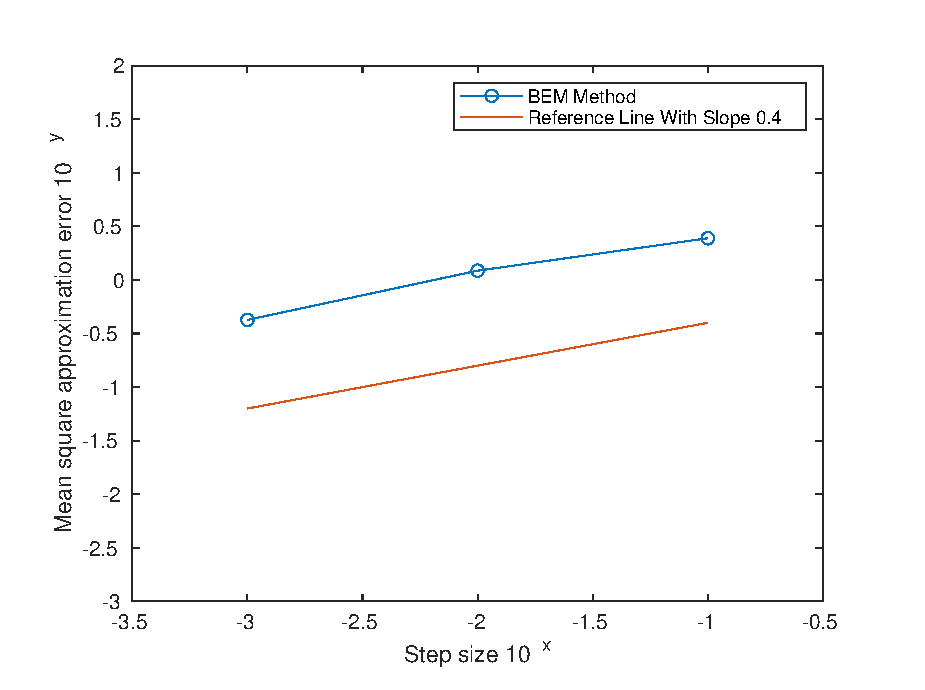
\includegraphics[width=0.45\linewidth]{alpha=0.4.eps}
			\hfill
			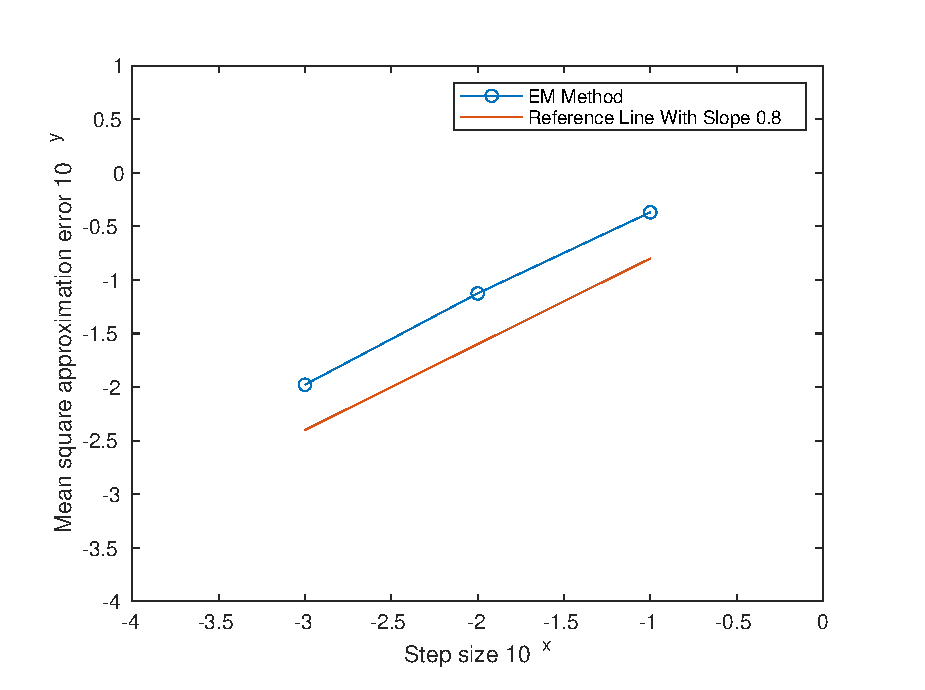
\includegraphics[width=0.45\linewidth]{alpha=0.8.eps}
			\caption{EM方法的$L_1$误差,左图为$\alpha=0.4$,右图为$\alpha=0.8$}
			\label{fig:image}
			\vspace{-2ex}
			{}\end{figure}



	
%	\section{Present problems}
%	\subsection{尝试使用更小的步长模拟D,看$\alpha=0.1$能否得到好的数值结果}
%	从优化后代码来看,模拟1000条轨道,将$2^{-16}$作为参考步长,从$2^{-5},2^{-6},2^{-7},2^{-8}$步长的结果是当$\alpha=0.1$,对应的收敛阶是0.1181
%	\subsection{关于一些等式不等式是否能够直接应用到时间变换上面}
%	3.尝试解决这个问题:
%	\begin{align}
%		\mathbb{E}(dB_EdE)^{q}\sim\Delta t^{(\frac{1}{2}+\alpha)q}\\\mathbb{E}(dEdE)^{q}\sim\Delta t^{(1+\alpha)q}
%	\end{align}
%	但是越来越觉得只能使用$L_1$误差了.2024.07.04代码模拟的结果是可以做到任何的$L^p$误差\\
%	4.之前给老师模拟的drift是超线性的例子,我使用的还是EM方法,但是这个时候就是会发散的呀,现在来看,爆炸是很正常的事情,后面尝试一下BEM能不能得到收敛?  \\
%	5.在数值模拟时,dBE期望算出来的不是0.5而是0.7左右,dBEdE算出来的是$0.7+\alpha$,但是理论计算可以得到dBE期望是0.5,dBEdE期望是$0.5+\alpha$,这样不会影响理论结果是$\alpha$,但是数值结果看起来并不是$c_1h^\alpha + c2h^\alpha$,而是$c_1h^\alpha + c_2h^{\alpha+\xi}$,其中$\xi$大概是0.1,尽管数值模拟是这样子的,但是这个貌似不会影响SDE解的模拟,因为$c_1h^\alpha + c_2h^{\alpha+\xi} \le c_1h^\alpha + c_2h^{\alpha}$是成立的
	
	
	
%	% 开始附录部分
%	\appendix
%	\renewcommand{\appendixname}{附录} % 自定义附录标题
%	\section{附录A}\label{appendix A}
	
	%%%%%%%%%%%%%%%%% 生成参考文献 %%%%%%%%%%%%%%%%%%%%%
	
	%\nocite{*}  % 可以暂时显示全部参考文献
	\bibliographystyle{plain}
	\bibliography{reference}
	
	
	
	
\end{document}

